\documentclass[]{elsarticle} %review=doublespace preprint=single 5p=2 column
%%% Begin My package additions %%%%%%%%%%%%%%%%%%%
\usepackage[hyphens]{url}

  \journal{Forest Ecology and Management} % Sets Journal name


\usepackage{lineno} % add
\providecommand{\tightlist}{%
  \setlength{\itemsep}{0pt}\setlength{\parskip}{0pt}}

\usepackage{graphicx}
\usepackage{booktabs} % book-quality tables
%%%%%%%%%%%%%%%% end my additions to header

\usepackage[T1]{fontenc}
\usepackage{lmodern}
\usepackage{amssymb,amsmath}
\usepackage{ifxetex,ifluatex}
\usepackage{fixltx2e} % provides \textsubscript
% use upquote if available, for straight quotes in verbatim environments
\IfFileExists{upquote.sty}{\usepackage{upquote}}{}
\ifnum 0\ifxetex 1\fi\ifluatex 1\fi=0 % if pdftex
  \usepackage[utf8]{inputenc}
\else % if luatex or xelatex
  \usepackage{fontspec}
  \ifxetex
    \usepackage{xltxtra,xunicode}
  \fi
  \defaultfontfeatures{Mapping=tex-text,Scale=MatchLowercase}
  \newcommand{\euro}{€}
\fi
% use microtype if available
\IfFileExists{microtype.sty}{\usepackage{microtype}}{}
\bibliographystyle{elsarticle-harv}
\usepackage{graphicx}
% We will generate all images so they have a width \maxwidth. This means
% that they will get their normal width if they fit onto the page, but
% are scaled down if they would overflow the margins.
\makeatletter
\def\maxwidth{\ifdim\Gin@nat@width>\linewidth\linewidth
\else\Gin@nat@width\fi}
\makeatother
\let\Oldincludegraphics\includegraphics
\renewcommand{\includegraphics}[1]{\Oldincludegraphics[width=\maxwidth]{#1}}
\ifxetex
  \usepackage[setpagesize=false, % page size defined by xetex
              unicode=false, % unicode breaks when used with xetex
              xetex]{hyperref}
\else
  \usepackage[unicode=true]{hyperref}
\fi
\hypersetup{breaklinks=true,
            bookmarks=true,
            pdfauthor={},
            pdftitle={How restrictions of forest management affect landscape level wind damage risk},
            colorlinks=false,
            urlcolor=blue,
            linkcolor=magenta,
            pdfborder={0 0 0}}
\urlstyle{same}  % don't use monospace font for urls

\setcounter{secnumdepth}{0}
% Pandoc toggle for numbering sections (defaults to be off)
\setcounter{secnumdepth}{0}


% Pandoc header



\begin{document}
\begin{frontmatter}

  \title{How restrictions of forest management affect landscape level wind damage
risk}
    \author[Department of Biological and Environmental Science]{Mária Potterf\corref{1}}
   \ead{mpotterf@jyu.fi} 
    \author[Department of Biological and Environmental Science]{Kyle Eyvindson}
   \ead{kyle.j.eyvindson@jyu.fi} 
    \author[Department of Biological and Environmental Science]{Clemens Blattert}
   \ead{clemens.c.blattert@jyu.fi} 
    \author[Department of Biological and Environmental Science]{Daniel Burgas}
   \ead{daniel.d.burgas-riera@jyu.fi} 
    \author[Department of Biological and Environmental Science]{Mikko Mönkkönen}
   \ead{mikko.monkkonen@jyu.fi} 
      \address[University of Jyvaskyla]{Department of Biological and Environmental Science, University of
Jyvaskyla, P.O. Box 35, FI-40014 Jyvaskyla, Finland}
    \address[Wisdom]{This is wisdom address}
    \address[LUKE]{THIS is Luke address Department, Street, City, State, Zip}
      \cortext[1]{Corresponding Author}
    \cortext[]{}
  
  \begin{abstract}
  Current forest management seeks to reconside timber harvesting while
  aims to improve forest diversity and halt biodiversity loss. Novel
  approaches as optimization of forest management regimes, increasing
  proportion of set-aside forest stands, or novel management approaches
  such as continuous forest cover emerge. However, novel ways of forest
  management shape structures of the forest stands over the landscape
  which will in turn affect the vulnerability to resist to more frequent
  climatic disruptions, such as windthrows. To understand how will the
  traditional (rotation forestry, RF) and novel forest managements
  techniques (continuous cover forest, CCF) alternate the risk of wind
  damages over the harvest intensity gradient (ranging from completely
  setaside to highest harvesting rates), we combined the forest growth
  simulator under ranges of management regimes (RF, CCF and combined:
  ALL), optimized over the range of harvesting levels to calculate stand
  and landscape level wind damage risk for alternative paths of the forest
  management and harvesting levles over 100 years. We found that higher
  harvest intensity in RF lowers wind risk, whereas the wind risk
  increased under CCF and ALL scenarios. More intensive harvesting using
  RF produced more pulp, while CCF provided higher volumes of the standing
  and harvested log wood, which likely explains higher values of wind risk
  probability. RF slightly increased the number of stands with open edge,
  which remained stable under CCF and ALL regimes. Intensive harvesting
  may change species composition to favour Norway spruce which will
  further increase probability of wind damage in the future. Therefore, we
  suggest that forest managers should consider the target forest species
  composition to mitigate wind risk if aimed to support production of log
  wood over the pulp.
  \end{abstract}
  
 \end{frontmatter}

\newpage

\section{Introduction}\label{introduction}

Adaptive forest management aims to balance between forest productivity,
provision of non-woody ecosystem services, and biodiversity. Existance
of biodiversity, mostly attached to existence of deadwood, is limited by
harvesting levels. Intensive logging activities fragment forested
landspaces. To balance between biodiversity and economic gain from
timber, the propostion of set=aside forests within commercial forests
emerges, and new forest management approaches are explored, such as
continuous forest cover (Eyvindson et al., 2021) and traditional
harvesting regimes are becoming controversial or requested to ban
(\ldots{}). The increase of the set aside forests within the commercial
forests, as well as development of the new management techniques affect
landscape level structural diversity, timing of the thinning, presence
of absence of the final cuts in rotation forestry or development of the
larger trees within continuous cover forestry or in set-aside forestry.
The fundamental is the carefull landscape level planning of the
management actions balancing between set-aside (unmanaged forests),
intensive management and continuously present forest cover.

Optimal management scenarios fullfil the specific objectives of the
society of forest owners to provide certain timber value, improve
provision of timber and non-timber ecosystem services, or improve
overall forest multifunctionality of the landscape. As such,
optimization provides the combination of the specific forest management
regimes on stand level. Althought the optimization process does not
necessary involve the spatial configuration of the stands, it
specifically assigns the particular regimes to individual stands and
therefore allows to recreate alternative dynamics landscapes shaped by
forest managements aggregated by optimal scenarios. As such, the spatial
configuration of the management regimes allows to estimate the
subsequent characteristics such as landscape level risk of wind damage.

The risk of the wind damage increases with current climate change and it
creates the major risk to the stability of the forest production.
Windthrows are unpredictable climatic disruption that shapes forest
structure and composition, and if left unsalvaged could create
opportiunities for deadwood dependent species and support local
biodiversity. From economical point of view, however, windthrows
massively abrupt the continuity of the timber supply, lowers timber
quality from log to pulp, increases the prices of unplanned salvage
harvesting (REF). To lower the risk of wind risk damage, current
suggestions include shortening the rotation period, promoting/avoiding
the wind resistant vs.~wind prone tree specuies, advocate for shortening
of the minimal stand age (Latvia REF). This however poses further
pressure on the multifucntionnal and multiple objective oriented
landscapes, which will provide habitats for endangered species, support
non-timber services and forest recreational use.

Traditional forest management regimes specialized in promoting timber
revenues while minimizing costs. In Fennoscandia, over the decades, the
traditional rotation forestry with multiple thinnings and final cuts
that over just mutlipel decades (from 1950) homogenized stands
structureal diversity, homogenized landscapes and increased forest
fragmenetations. On the other hand, forest management supporting
multifunctional landscapes, and promoting non-timber ecosystem services
requires implementation of the diverse set of management regimes
(Mönkkönen et al., 2014; Triviño et al., 2017). Furthermore, provision
of the endangered species habitats and non-woody ecosystem services are
provided on different scales where the planning scale should match or
overcome the scale that provided ecosystem (Pohjanmies et al., 2019).

Here we explore how the restriction of forest management practices,
along with the increasing level of harvest levels over the landscape
affects landscape level damage of wind risk and how much timber value is
put on risk under alternative regimes and extraction levels. Our study
for the first time evaluates the landcspeca level wind risk combined
with the forest growth simulator and long-term consequences of he
applied forest management practices. Therefore, we first calculate the
stand level wind risk over alternative landscapes and further explore
the likely drivers of the wind risk levels. We investigated how
restriction of forest management regimes combined with levels of
intensity of timber extraction will affects landscape level wind risk.

We hypothesized that RF would increase wind damage risk dues to
increasing number of open edges while CCF would lower wind risk over the
landscape. Further, we hypothetize that higher levels of timber
extraction would increase wind risk. Lastly, we hypothetized than
increasing amount of set-aside stands, over the landscape together with
CCF management would increase wind damage risk due to larger present
timber volume, and due to more frequent thinning activities. We
investigated wind risk in terms of available timber volume, specifically
saw and log timber volume. Lastly, we explored the trends of wind risk
relevant to stands height, changes and species compositions.

\section{Methods}\label{methods}

\paragraph{Study area}\label{study-area}

Our study area represents a typical Finnish production forested
landscape with relatively structurally homogenous forests stands. In
total, we used 1475 forests stands aggregated within a single watershed
(number 14.534) in Central Finland, covering 2242 ha (Fig.
\ref{study_area}). Initial stand conditions were collected as open
source data from the Finnish Forest Centre (available on www.metsaan.fi)
providing currents stand conditions in 2016.

Our input dataset includes initial stand conditions (2016), alternative
forest growth under the range of forest managemnet regimes over 100
years and a set of optimal solutions balancing between intensifying
harvest levels and multifunctionnality (from completely set-aside,
i.e.~no management to maximal harvest gains). From the set of optimal
solutions we have calculated stand-level probability of wind damage (for
full details, please refer to Eyvindson et al. (2021) study (Fig.
\ref{workflow})).

\begin{figure}
\centering
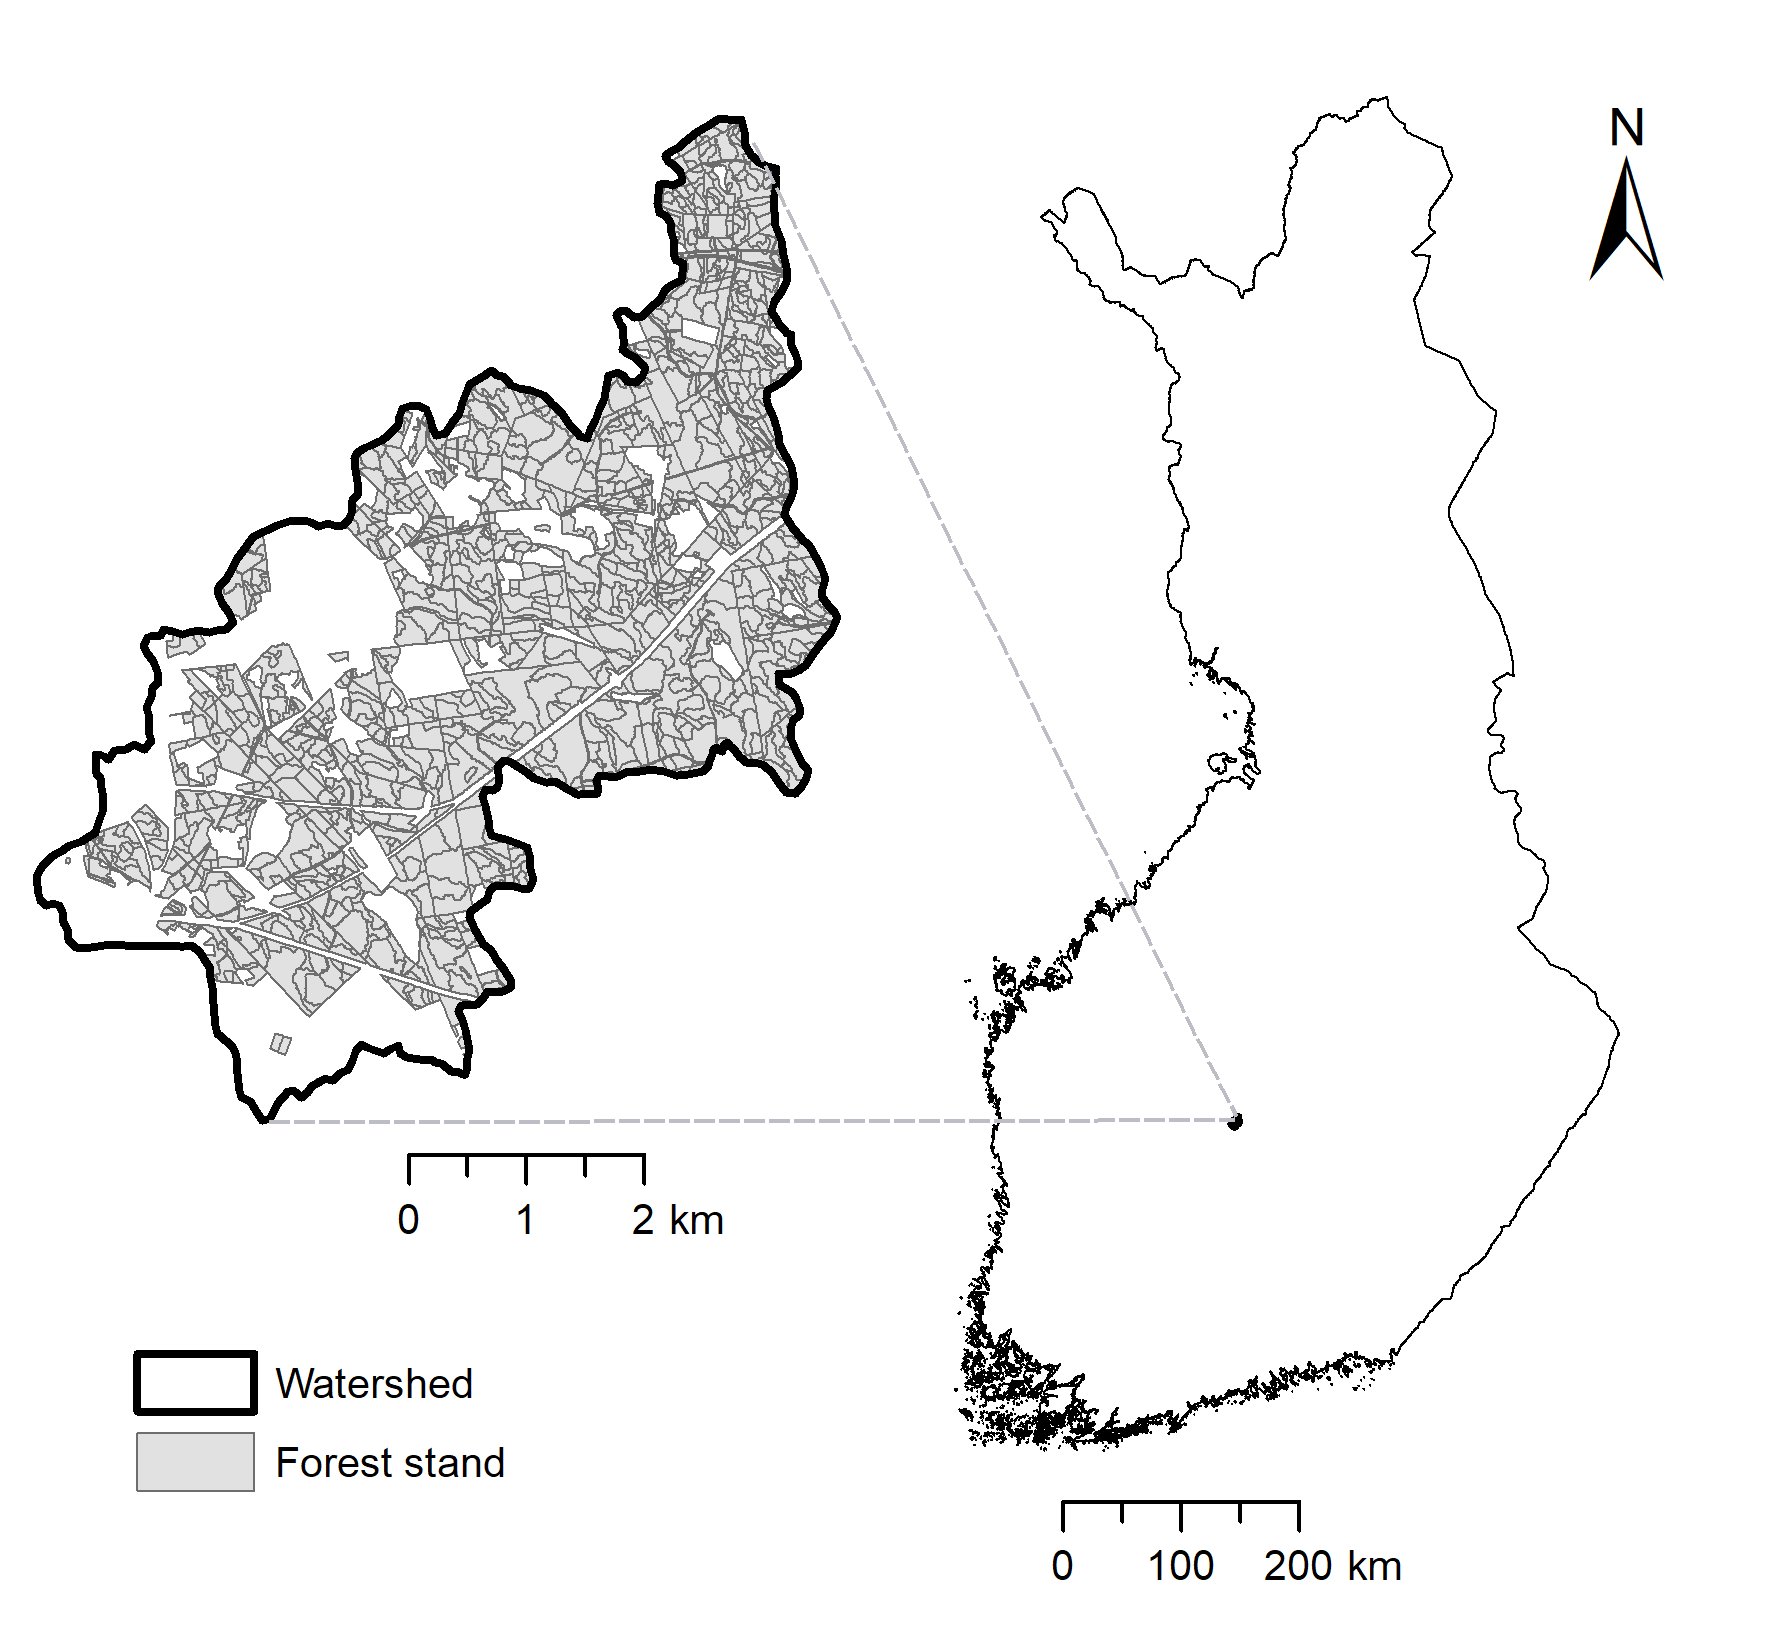
\includegraphics{/MyTemp/myGitLab/windDamage/externalFigs/studyArea_crop.png}
\caption{The study area located in Central Finland (watershed 14.534)
comprising 1475 forest stands.\label{study_area}}
\end{figure}

\begin{figure}
\centering
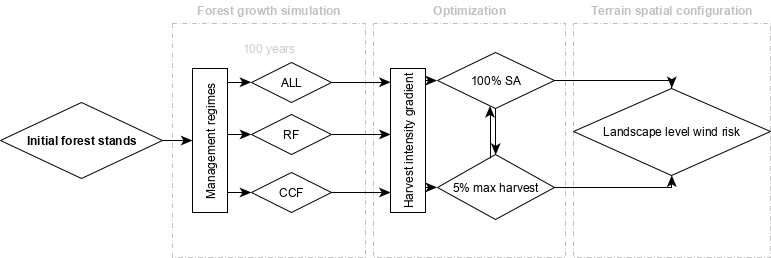
\includegraphics{/MyTemp/myGitLab/windDamage/externalFigs/overview2_horizontal.png}
\caption{The study workflow from collecting initial stand conditions
(2016) throught forest simulation growth under various ranges of forest
management, and constriuction of teh harvesting intensity gradient using
optimization to landscape level stand configurations.\label{workflow}}
\end{figure}

\paragraph{Forest stand development under different
regimes}\label{forest-stand-development-under-different-regimes}

We simulated the development of the forests stands using SIMO forest
growth simulator ({\textbf{???}}) over 100 years, separated into 20
5-year sequences. Each stand could be managed by up to 58 different
management regimes (the total number of regimes per stands depended on
the initial stand conditions), including 17 regimes for rotation
forestry (RF), 40 variations of continuous cover forest (CCF) and one
set-aside (SA), where no management actions were taken. RF regimes
differed in timing of final felling, optional thinning (present/absent),
and increase in number of retained green trees after final cut (more
details in Eyvindson and Kangas (2018)). Basic CCF management follows
rules from Äijälä et al. (2014). To increase the range of CCF
managements, we varied two rules defining the timing of harvest: (i)
site-specific basal area and (ii) timing of the first thinning. We
modified the pre-defined site-specific basal area requirement (16m2/ha
for less fertile sites to 22m2/ha for fertile sites) prior to harvesting
by -3, ±0, +3, +6, and delayed the timing of the first harvest in 5 year
increments up to a delay of 45 years.

\paragraph{Optimization}\label{optimization}

The optimal forest management explores the trade-offs between net
present income (NPI) and forest multifunctionality. NPI represents
economic value of the forests estimated by Metsähallitus (the Finnish
governmental organization managing state owned forests). Higher NPI
presents higher timber extraction and opposes the proportion of the
set-aside forest stands (i.e.~without active harvesting) over the
landscape. Optimization process over the NPI gradient was run using only
RF, only CCF management types, or all possible managements (RF and CCF,
further reffered as ALL) included over the gradient of NPI values, from
0 (representing completely set-aside or no management in all stands) to
maximal amount of extracted timber (leaving up to 5\% of SA stands). The
optimization balances between harvest intensity and landscape-level
multifunctionnality, including non-woody ecosystem services (climate
change mitigation), recreational activities and vertebrate and
non-vertebrate endangered species. The optimization resulted in 63
alternative collections of RF, CCF and ALL manamement regimes. We
converted the optimal solutions back to the development paths for every
stand under alternative management given group of management allowed
(CCF, RF, ALL) and levels of timber extraction (21). Each stand has only
one management regime by scenario. This allowed to reconstruct stand
structure on particular stand under given management regime at specific
time.

\paragraph{Wind risk calculation}\label{wind-risk-calculation}

We have calculated the probability of wind damage based on Suvanto et
al. (2019) binomial generalized linear model with logit-link function
for each stand for every time step at each scenario. Suvanto et al.
(2019) model calculates the probability of the wind damage considering
available relevant open-access datasets including dominant tree species,
dominant tree height, time since thinning, predicted levels on maximal
wind speed, temperature sums, evaluated if stand has open edge, soil
type, mineral soil depth, site fertility and temperature sum (see
Suvanto et al. (2019) for all details). The final probability of wind
damage shows relative differences between stands, whereas the damage can
be only partial to the stand, but neglects the explicit spatial
locations of the future strongs winds. The parameters of the dominant
tree species, tree height, open edge and time since thinning were
dynamics under simulated management regimes. Parameters of maximal
predicted wind speed and temperature sums, as well as soil
characteristics, remained stable during our 100 years simulation. We
processed the datasets, calculated damage probability models, and
visualized results using R Development Core Team (2019).

\paragraph{Data processing}\label{data-processing}

We calculated the probability of wind damage for each stand, scenario
and time intervals. Further, we averaged the wind risk values over the
scenarios to allow comparison between RF, CCF and ALL management regimes
groups over the harvesting gradient. We explored the mean wind risk (\%)
given the management groups and over harvest gradient (from set-aside to
maximal harvest levels). In addition, we investigated the mean levels of
the standing log and pulp timber volumes (m3) for scenarios, and total
sum of harvested pulp and log timber over simulation run (XXX). We
further investigated the means of dynamic parameters (tree species,
dominant tree height, frequency of open edges and time since thinning)
over the harvest intensity gradient to understand how they contributed
to predicted wind risk values.

\section{Results}\label{results}

\paragraph{Landscape level wind risk under management restriction and
harvest intensity
scenarios}\label{landscape-level-wind-risk-under-management-restriction-and-harvest-intensity-scenarios}

The set-aside landscape level management resulted at the same mean
landscape level risk for all management regimes (Fig. 2). However,
intensifying harvesting triggers different responses under groups of
management regimes and intensification of the timber extraction. Sole
use of the RF managements lowered the wind risk with increasing harvest
intensity. On the other hand, both ALL and CCF scenarios increased the
wind risk where CCF monotonically increased with increasing harvesting
rates, while ALL regimes have slightly humpened curve shape, culminating
around inteinsity of 7.5K by ha. The CCF increases monotonically while
maximal harvesting increase the wind risk by 25\% compared to completely
set-aside stands.

\begin{figure}
\centering
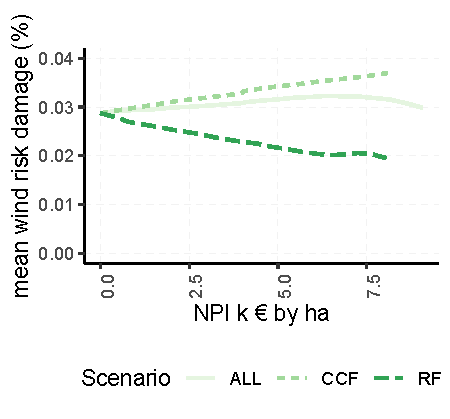
\includegraphics{test_manus_files/figure-latex/fig3_mean_risk_by_intensity_plot-1.pdf}
\caption{Mean wind risk damage for three types of management regimes
over harvest intensity gradient}
\end{figure}

\paragraph{Timber volume at wind risk}\label{timber-volume-at-wind-risk}

Increasing harvesting levels lowers the amount of the available timber
at any time step to be lost due to windthrows. Interestingly, the CCF
regimes produces higher logs volumes, while RF has higher production of
the pulp wood, which is in high demand by cheaper then log wood. The
same trends are visible for harvested log and pulp volumes. For ALL
management regimes, using all available management regimes, is located
between two extremities. The highest mean log timber volume as available
for the wind damage at lowest harvesting levels. Interestingly, under
RF, low levels of timber extraction increase levels of the pupl standing
volume. The highest amount of harvested log wood is produced by CCF
regimes, while RF dominates in harvesting pulp timber
@ref(fig:fig\_4\_plot\_V\_timber).

\begin{figure}
\centering
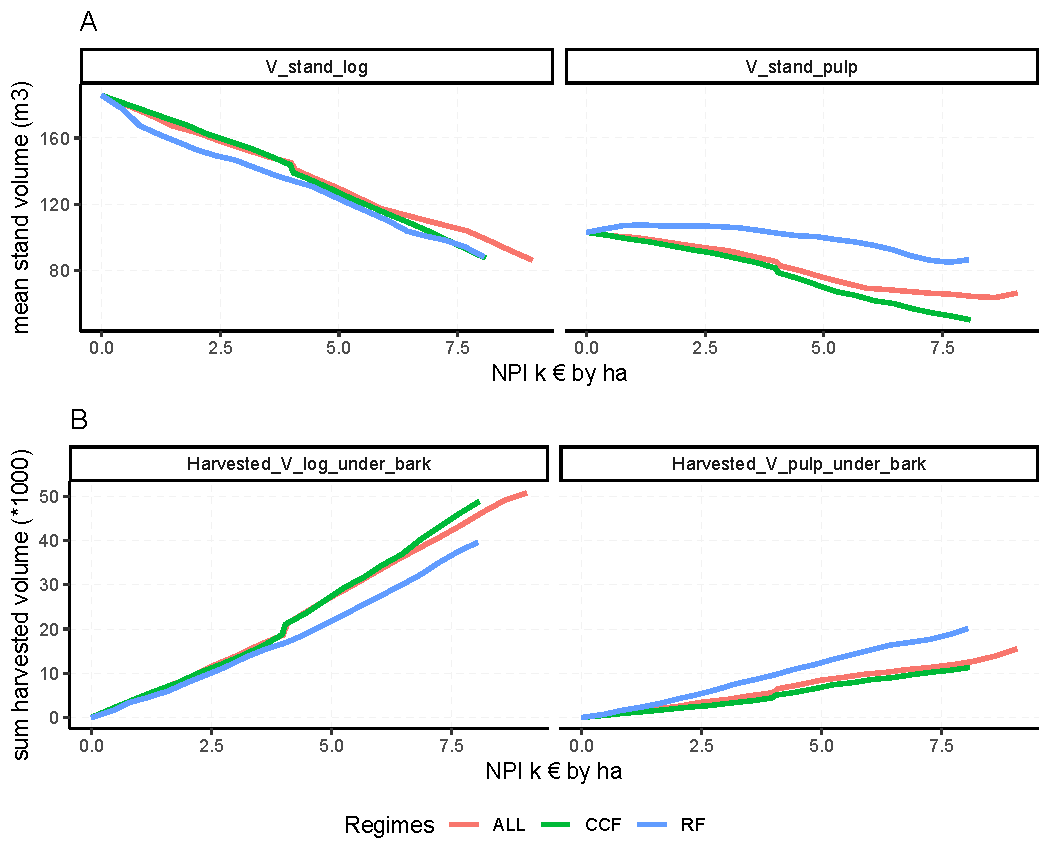
\includegraphics{test_manus_files/figure-latex/fig_4_plot_V_timber-1.pdf}
\caption{A. Mean standing and B. harvested pulp and log timber under
three types of management regimes over harvest intensity gradient}
\end{figure}

The intensification of the harvesting levels increases the proportion of
the pulp wood compared to log wood, especially in RF. In CCF, the
proportion among standing log and pulp volume remains at the same rate
(65:30) where the production of the log timber dominates. At the highest
intensity of timber extraction, pulp wood creates up to 50\% of teh
total standing volume See figure
@ref(fig:fig\_5\_proportion\_V\_pulp\_log) NEW FIG
@ref(fig\_5\_proportion\_V\_pulp\_log).

\subsubsection{Dynamic parameters contributing to wind
risk}\label{dynamic-parameters-contributing-to-wind-risk}

\paragraph{Species composition}\label{species-composition}

The intensification of the harvesting changes the stand species
composition over time (Fig. \ref{species_change}). Intensification of
the harvesting favorize the proportion of the Norway spruce and others
(deciduous) tree species instead of Scots pine, which likely in turn
increases wind risk over the stands.

\begin{figure}
\centering
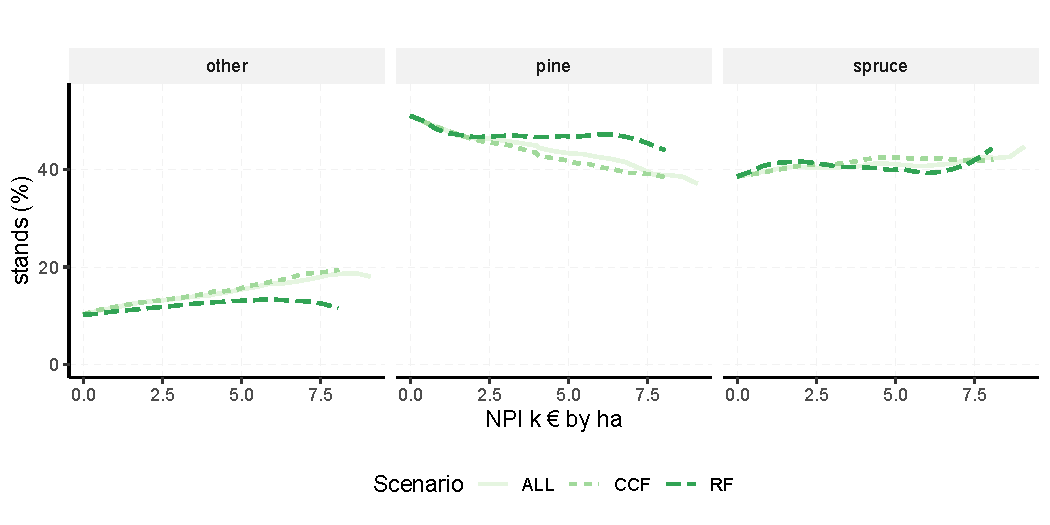
\includegraphics{test_manus_files/figure-latex/species_change-1.pdf}
\caption{Changes in species composition under different management
groups and harvest intensity. (The ALL scenario leads to highest
economic gain, tehrefore values for CCF and RF are missing from plot)}
\end{figure}

\paragraph{Dominant tree heights}\label{dominant-tree-heights}

The intensification of the harvesting changes the stand species
composition over time (Fig. \ref{species_change}). Intensification of
the harvesting favorize the proportion of the Norway spruce and others
(deciduous) tree species instead of Scots pine, which likely in turn
increases wind risk over the stands.

\begin{figure}
\centering
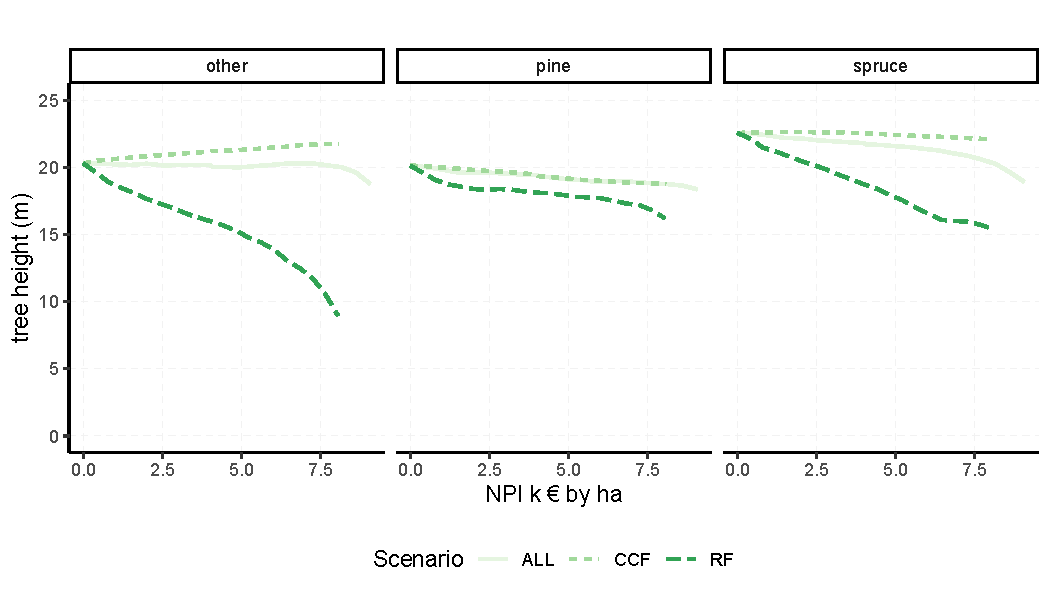
\includegraphics{test_manus_files/figure-latex/res_D_tree_height-1.pdf}
\caption{Mean dominant tree height under different management groups and
harvest intensity.}
\end{figure}

\paragraph{Frequency of open stands}\label{frequency-of-open-stands}

RF regimes increase the amount of stands with open edge with increasing
harvest intensity while CCF regimes maintain the same amount of open
stands over the harvest intensity gradient. Intensive RF increases
number of stands with open edge by 5\%.

\begin{figure}
\centering
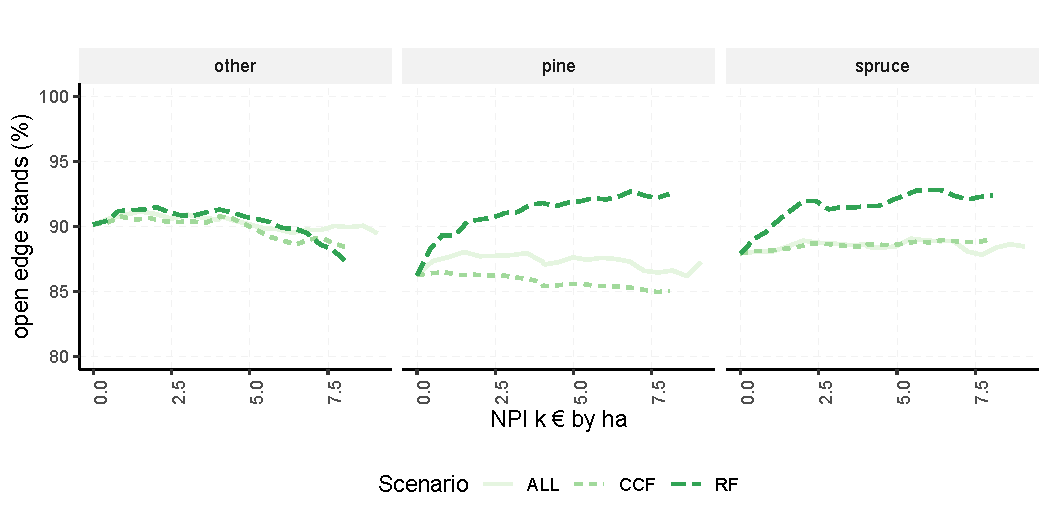
\includegraphics{test_manus_files/figure-latex/fig_6_count_open_edge-1.pdf}
\caption{Yearly count of stands with open edge over the intensity
gradient}
\end{figure}

\paragraph{Thinning frequency}\label{thinning-frequency}

\begin{verbatim}
##                id year Age cash_flow       BA        V V_stand_log V_stand_pulp
##       1: 12515084 2016  51         0 15.92991 121.9846    50.43912     69.03075
##       2: 12515084 2021  56         0 15.97570 122.4578    50.81278     69.09368
##       3: 12515084 2026  61         0 16.02149 122.9315    50.94787     69.39531
##       4: 12515084 2031  66         0 16.06730 123.4057    51.08273     69.69723
##       5: 12515084 2036  71         0 16.11311 123.8802    51.21737     70.11885
##      ---                                                                       
## 1852196:  6691970 2091 165         0 14.02046 149.2695   126.53544     21.80980
## 1852197:  6691970 2096 170         0 13.75152 146.9029   126.40365     19.62537
## 1852198:  6691970 2101 175         0 13.57640 145.4288   125.87290     18.73834
## 1852199:  6691970 2106 180         0 13.47255 144.6260   125.76314     18.08305
## 1852200:  6691970 2111 185         0 13.42110 144.3109   126.50326     17.01734
##          Harvested_V Harvested_V_log_under_bark Harvested_V_pulp_under_bark
##       1:           0                          0                           0
##       2:           0                          0                           0
##       3:           0                          0                           0
##       4:           0                          0                           0
##       5:           0                          0                           0
##      ---                                                                   
## 1852196:           0                          0                           0
## 1852197:           0                          0                           0
## 1852198:           0                          0                           0
## 1852199:           0                          0                           0
## 1852200:           0                          0                           0
##          Biomass        N THIN PEAT    H_dom     D_gm income_biomass
##       1:       0 697.8802 <NA>    1 167.9335 18.70460              0
##       2:       0 696.3087 <NA>    1 168.1394 18.73898              0
##       3:       0 694.7542 <NA>    1 168.3448 18.77329              0
##       4:       0 693.2163 <NA>    1 168.5497 18.80752              0
##       5:       0 691.6946 <NA>    1 168.7540 18.84168              0
##      ---                                                            
## 1852196:       0 251.7209 <NA>    0 260.0189 29.40783              0
## 1852197:       0 241.5970 <NA>    0 260.4277 29.55030              0
## 1852198:       0 233.8745 <NA>    0 260.8226 29.69387              0
## 1852199:       0 228.0484 <NA>    0 261.2026 29.83591              0
## 1852200:       0 223.6549 <NA>    0 261.5679 29.97626              0
##          CARBON_STORAGE name_new branching_new avohaakut THIN_included
##       1:             NA       SA          <NA>        SA         FALSE
##       2:             NA       SA          <NA>        SA         FALSE
##       3:             NA       SA          <NA>        SA         FALSE
##       4:             NA       SA          <NA>        SA         FALSE
##       5:             NA       SA          <NA>        SA         FALSE
##      ---                                                              
## 1852196:       267558.7       SA          <NA>        SA         FALSE
## 1852197:       262147.2       SA          <NA>        SA         FALSE
## 1852198:       256662.0       SA          <NA>        SA         FALSE
## 1852199:       251972.7       SA          <NA>        SA         FALSE
## 1852200:       247921.1       SA          <NA>        SA         FALSE
##          mainRegime scenSimpl2 scenNumb landscape difference time_thinning
##       1:         SA        ALL        0 2016_ALL0         NA           >10
##       2:         SA        ALL        0 2021_ALL0         NA           >10
##       3:         SA        ALL        0 2026_ALL0         NA           >10
##       4:         SA        ALL        0 2031_ALL0         NA           >10
##       5:         SA        ALL        0 2036_ALL0         NA           >10
##      ---                                                                  
## 1852196:         SA         RF        9  2091_RF9         NA           >10
## 1852197:         SA         RF        9  2096_RF9         NA           >10
## 1852198:         SA         RF        9  2101_RF9         NA           >10
## 1852199:         SA         RF        9  2106_RF9         NA           >10
## 1852200:         SA         RF        9  2111_RF9         NA           >10
##          avoh_Simpl simpleScen open_edge      area siteFertility
##       1:         SA        ALL      TRUE 10218.091          poor
##       2:         SA        ALL      TRUE 10218.091          poor
##       3:         SA        ALL      TRUE 10218.091          poor
##       4:         SA        ALL      TRUE 10218.091          poor
##       5:         SA        ALL      TRUE 10218.091          poor
##      ---                                                        
## 1852196:         SA         RF      TRUE  2479.115       fertile
## 1852197:         SA         RF      TRUE  2479.115       fertile
## 1852198:         SA         RF      TRUE  2479.115       fertile
## 1852199:         SA         RF      TRUE  2479.115       fertile
## 1852200:         SA         RF      TRUE  2479.115       fertile
##          soilDepthLess30       soilType species   windRisk twoRegm      NPI
##       1:           FALSE        organic    pine 0.02327795      SA 0.000000
##       2:           FALSE        organic    pine 0.02332427      SA 0.000000
##       3:           FALSE        organic    pine 0.02337051      SA 0.000000
##       4:           FALSE        organic    pine 0.02341666      SA 0.000000
##       5:           FALSE        organic    pine 0.02346272      SA 0.000000
##      ---                                                                   
## 1852196:           FALSE mineral coarse  spruce 0.05105826      SA 3.622254
## 1852197:           FALSE mineral coarse  spruce 0.05130966      SA 3.622254
## 1852198:           FALSE mineral coarse  spruce 0.05155323      SA 3.622254
## 1852199:           FALSE mineral coarse  spruce 0.05178835      SA 3.622254
## 1852200:           FALSE mineral coarse  spruce 0.05201497      SA 3.622254
##               MF stands_n   SA_prop THIN2
##       1: 1.81712     1470 100.00000  <NA>
##       2: 1.81712     1470 100.00000  <NA>
##       3: 1.81712     1470 100.00000  <NA>
##       4: 1.81712     1470 100.00000  <NA>
##       5: 1.81712     1470 100.00000  <NA>
##      ---                                 
## 1852196: 1.74564      894  60.81633  <NA>
## 1852197: 1.74564      894  60.81633  <NA>
## 1852198: 1.74564      894  60.81633  <NA>
## 1852199: 1.74564      894  60.81633  <NA>
## 1852200: 1.74564      894  60.81633  <NA>
\end{verbatim}

\begin{figure}
\centering
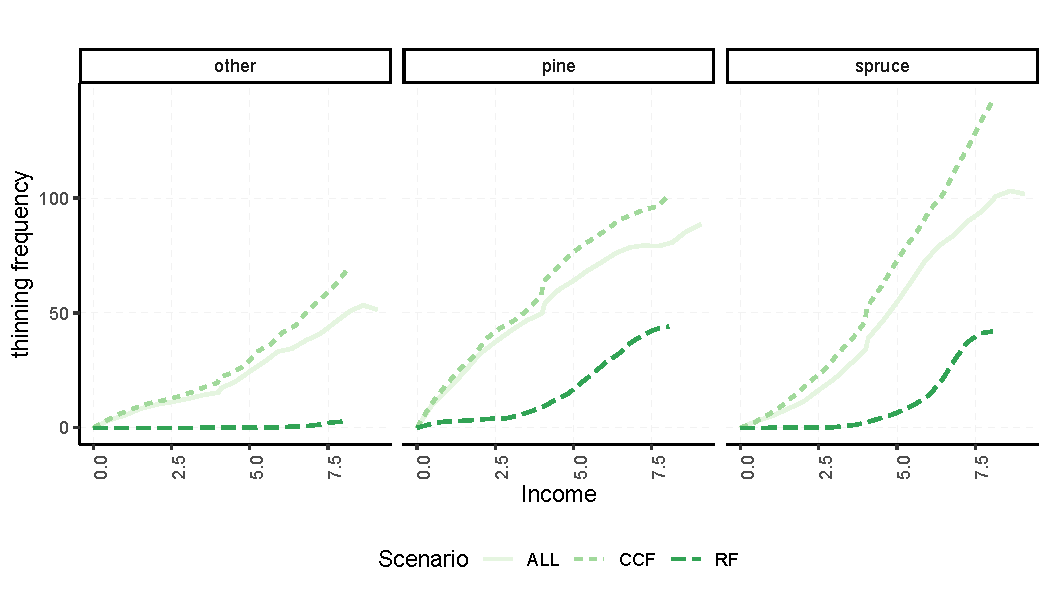
\includegraphics{test_manus_files/figure-latex/fig_thin_frequency-1.pdf}
\caption{THe frequency of the thinnings by management groups, species
and harvest intensity gradient}
\end{figure}

\section{Discussion}\label{discussion}

Wind (10 years return level of max wind speed REF) are estimated the
same over 100 years as well as temperature sums. How does could affects
the results?

In spite of inherent stochasticity of the wind and damage phenomena at
all spatial scales can be successfully modelled combining spatial
spatial datasets and ground earth observation data (Suvanto et al.
2019). Interpret Suvanto's map: there are 3 limitations: use values as
relative to each other - instead of exact probability valuesm, interpret
the map as relative differences in damage vulnerability Damage
probabilities do not refer to complete damage of the stand -- damage can
be only poartial, in some part of the stand (not spatially expicit) map
erepresent the forest vulnerability to the wind, but it is impossible to
predict the exact locations of future wind disturbances, given
uncertainities in future wind occurences

\section*{References}\label{references}
\addcontentsline{toc}{section}{References}

\hypertarget{refs}{}
\hypertarget{ref-Aijala2014a}{}
Äijälä, O., Koistinen, A., Sved, J., Vanhatalo, K., Väisänen, P., 2014.
Metsänhoidon suositukset {[}Good forest management recommendations{]}.
Forestry Development Center Tapio.

\hypertarget{ref-Eyvindson2020}{}
Eyvindson, K., Duflot, R., Triviño, M., Blattert, C., Potterf, M.,
Mönkkönen, M., 2021. High boreal forest multifunctionality requires
continuous cover forestry as a dominant management. Land Use Policy 100,
1--10.
doi:\href{https://doi.org/10.1016/j.landusepol.2020.104918}{10.1016/j.landusepol.2020.104918}

\hypertarget{ref-Eyvindson2018}{}
Eyvindson, K., Kangas, A., 2018. Guidelines for risk management in
forest planning --- what is risk and when is risk management useful?
Canadian Journal of Forest Research 48, 309--316.
doi:\href{https://doi.org/10.1139/cjfr-2017-0251}{10.1139/cjfr-2017-0251}

\hypertarget{ref-RDevelopmentCoreTeam2019}{}
R Development Core Team, 2019. R: A language and environment for
statistical computing.

\hypertarget{ref-Suvanto2019}{}
Suvanto, S., Peltoniemi, M., Tuominen, S., Strandström, M., Lehtonen,
A., 2019. High-resolution mapping of forest vulnerability to wind for
disturbance-aware forestry. Forest Ecology and Management 453, 117619.
doi:\href{https://doi.org/10.1016/j.foreco.2019.117619}{10.1016/j.foreco.2019.117619}


\end{document}


